A digital platform that interfaces with analog signals is an effective and flexible instrumentation strategy for electrophysiology experiments that require arbitrary stimulation signals and recording action potentials.  A digital to analog converter (DAC) can convert a digitally represented waveform to an analog signal that can be used to stimulate experimental subjects, and a analog to digital converter (ADC) can convert analog voltages to digital data that can be saved in readily available digital formats.

The user interface of the platform needs to be flexible to accommodate the various electrophysiology experiments it will perform.  Custom PC software allows the user to control the complex capabilities of the platform while also providing access to data storage space; however, PC hardware is not capable of interfacing directly with DAC and ADC circuits.  To save development complexity, real time control of the DAC and ADC is accomplished with a Digilent\textsuperscript{\textregistered} Nexys\textsuperscript{TM} 2 field-programmable gate array (FPGA) development board.  The DAC and ADC, along with related circuitry, are implemented on a custom designed printed circuit board (PCB).

An overview of the Data Acquisition and Stimulation System (DASS) is shown in Figure~\ref{fig:System}.  Custom user interface software on the PC communicates to the Digilent\textsuperscript{\textregistered} Nexys\textsuperscript{TM} 2 Real Time System Controller (RTSC) board over USB and serial RS232 interfaces.  An RS232 level converter chip converts the PC's RS232 logic levels to FPGA compatible TTL logic levels and vice-versa.  A microcontroller on the RTSC provides the USB physical layer (PHY) and is capable of controlling the Joint Test Action Group (JTAG) bus to load a FPGA configuration file into the FPGA or save the configuration to a flash memory device capable of storing the configuration on the board without power and loading the configuration into the FPGA upon power-up.  The JTAG bus also allows a configuration to be loaded into the Complex Programmable Logic Device (CPLD), which can be programmed with logic to allow the FPGA to control the multiple digital inputs on the Preamp boards with fewer output pins.  A DRAM chip on the RTSC stores stimulation waveform data.  The FPGA outputs stimulation waveform data to the DAC on the Electrophysiology Interface board and controls the ADC.  Data from the ADC is sent to the microcontroller, which has customized firmware that transfers data to the PC over the USB interface.

\begin{landscape}
\begin{figure} % [H] option tell Latex to place the figure at this place in the document
	\begin{singlespace}
	\centering	
		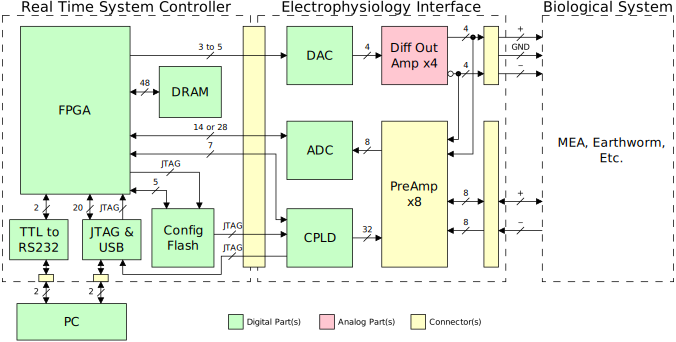
\includegraphics{./figures/System}
		% Tells (pdf)latex to look for graphic: System.*
		% running pdflatex will include System.pdf and running latex will include System.eps	
	\caption{The Data Acquisition and Stimulation System consists of a PC, the Real Time System Controller Board, which is a Digilent\textsuperscript{\textregistered} Nexys\textsuperscript{TM} 2 FPGA development board~\cite{DigilentNexys2rm,DigilentNexys2sch}, and the Electrophysiology Interface board, which is based on previous work as described in the text.\label{fig:System}}
	% \label{} allows this figure to be referenced in the text and it must be immediately after or in \caption{}
	\end{singlespace}
\end{figure}
\end{landscape}

The analog operating ranges of the DAC and ADC are not compatible with the voltages used in electrophysiology experiments, so a differential output amplifier circuit conditions the DAC output, and connectors are provided to allow previously developed low-noise amplifier boards~\cite{StahlMSEE} (Preamp) to condition low-voltage action potentials for input into the ADC.  The Preamp boards have the capability of outputting a provided analog stimulation signal on the recording electrode; digital inputs control whether the Preamp is in stimulation or recording mode.

Typical use of the DASS involves the following: connecting the Electrophysiology Interface board stimulation and data acquisition channels to the biological portion of the electrophysiology experimental setup; powering the Electrophysiology Interface and RTSC boards, which causes the FPGA to be configured based on the data in the flash memory configuration chip; using the PC application to send commands over the RS232 interface to the FPGA for configuring the stimulation and data acquisition channels~\cite{BatzerMSEE}; running a script on the PC application that sends commands to the FPGA over the RS232 interface to load stimulation waveform profiles in the DRAM, sets the Preamp boards to stimulation or recording mode, causes the DAC to output the stimulation waveform, collects data from the ADC, and transfers data collected from the ADC to the PC for storage and analysis~\cite{BatzerMSEE}.  Waveforms from the DAC output are amplified and conditioned by the Differential Output Amplifier before being routed to the biological system either to independent stimulation electrodes or through the Preamp boards to the recording electrodes.  The response from the biological system is observed on the recording electrodes as analog electrical signals which are routed to the Preamp boards for amplification and filtering before being routed to the ADC for conversion to digital information.

This thesis describes the relevant circuitry on a Digilent\textsuperscript{\textregistered} Nexys\textsuperscript{TM} 2 FPGA development board that is necessary to implement a RTSC board, and it describes the design of the Electrophysiology Interface board.  The design of the PC software, microcontroller firmware, and programmable logic configurations is described in~\cite{BatzerMSEE}.

